\section{Conclusiones} \label{conclusiones}
\AddToShipoutPictureBG*{
\includegraphics[width=\paperwidth,height=\paperheight]{Imagenes/Fondo Capitulo 2.pdf}}
\thispagestyle{plain}

\divider

El objetivo de este trabajo, diseñar, verificar y enviar a fabricar una placa de circuito impreso de una plataforma de evaluación, se logró concretar exitosamente dentro del plazo establecido, pasando por todas las fases del mismo, desde la lectura de hojas de datos y notas de aplicación pertinentes, la ubicación de componentes y el ruteo de las pistas que los conectan, la verificación de este diseño, y el contacto con algún fabricante de PCB. Así, se obtuvo una placa de doble capa sumamente compacta, de dimensiones de \SI[]{15}[]{\centi\metre} x \SI[]{16}[]{\centi\metre}, incluso a pesar de los inconvenientes en su diseño que se encontraron en el proceso. No solo esto, si no que el fabricante pudo fabricar cinco copias idénticas de la placa, una de las cuales se puede observar en la siguiente figura (sin sus componentes soldados).\\

\begin{figure}[h]
    \centering
    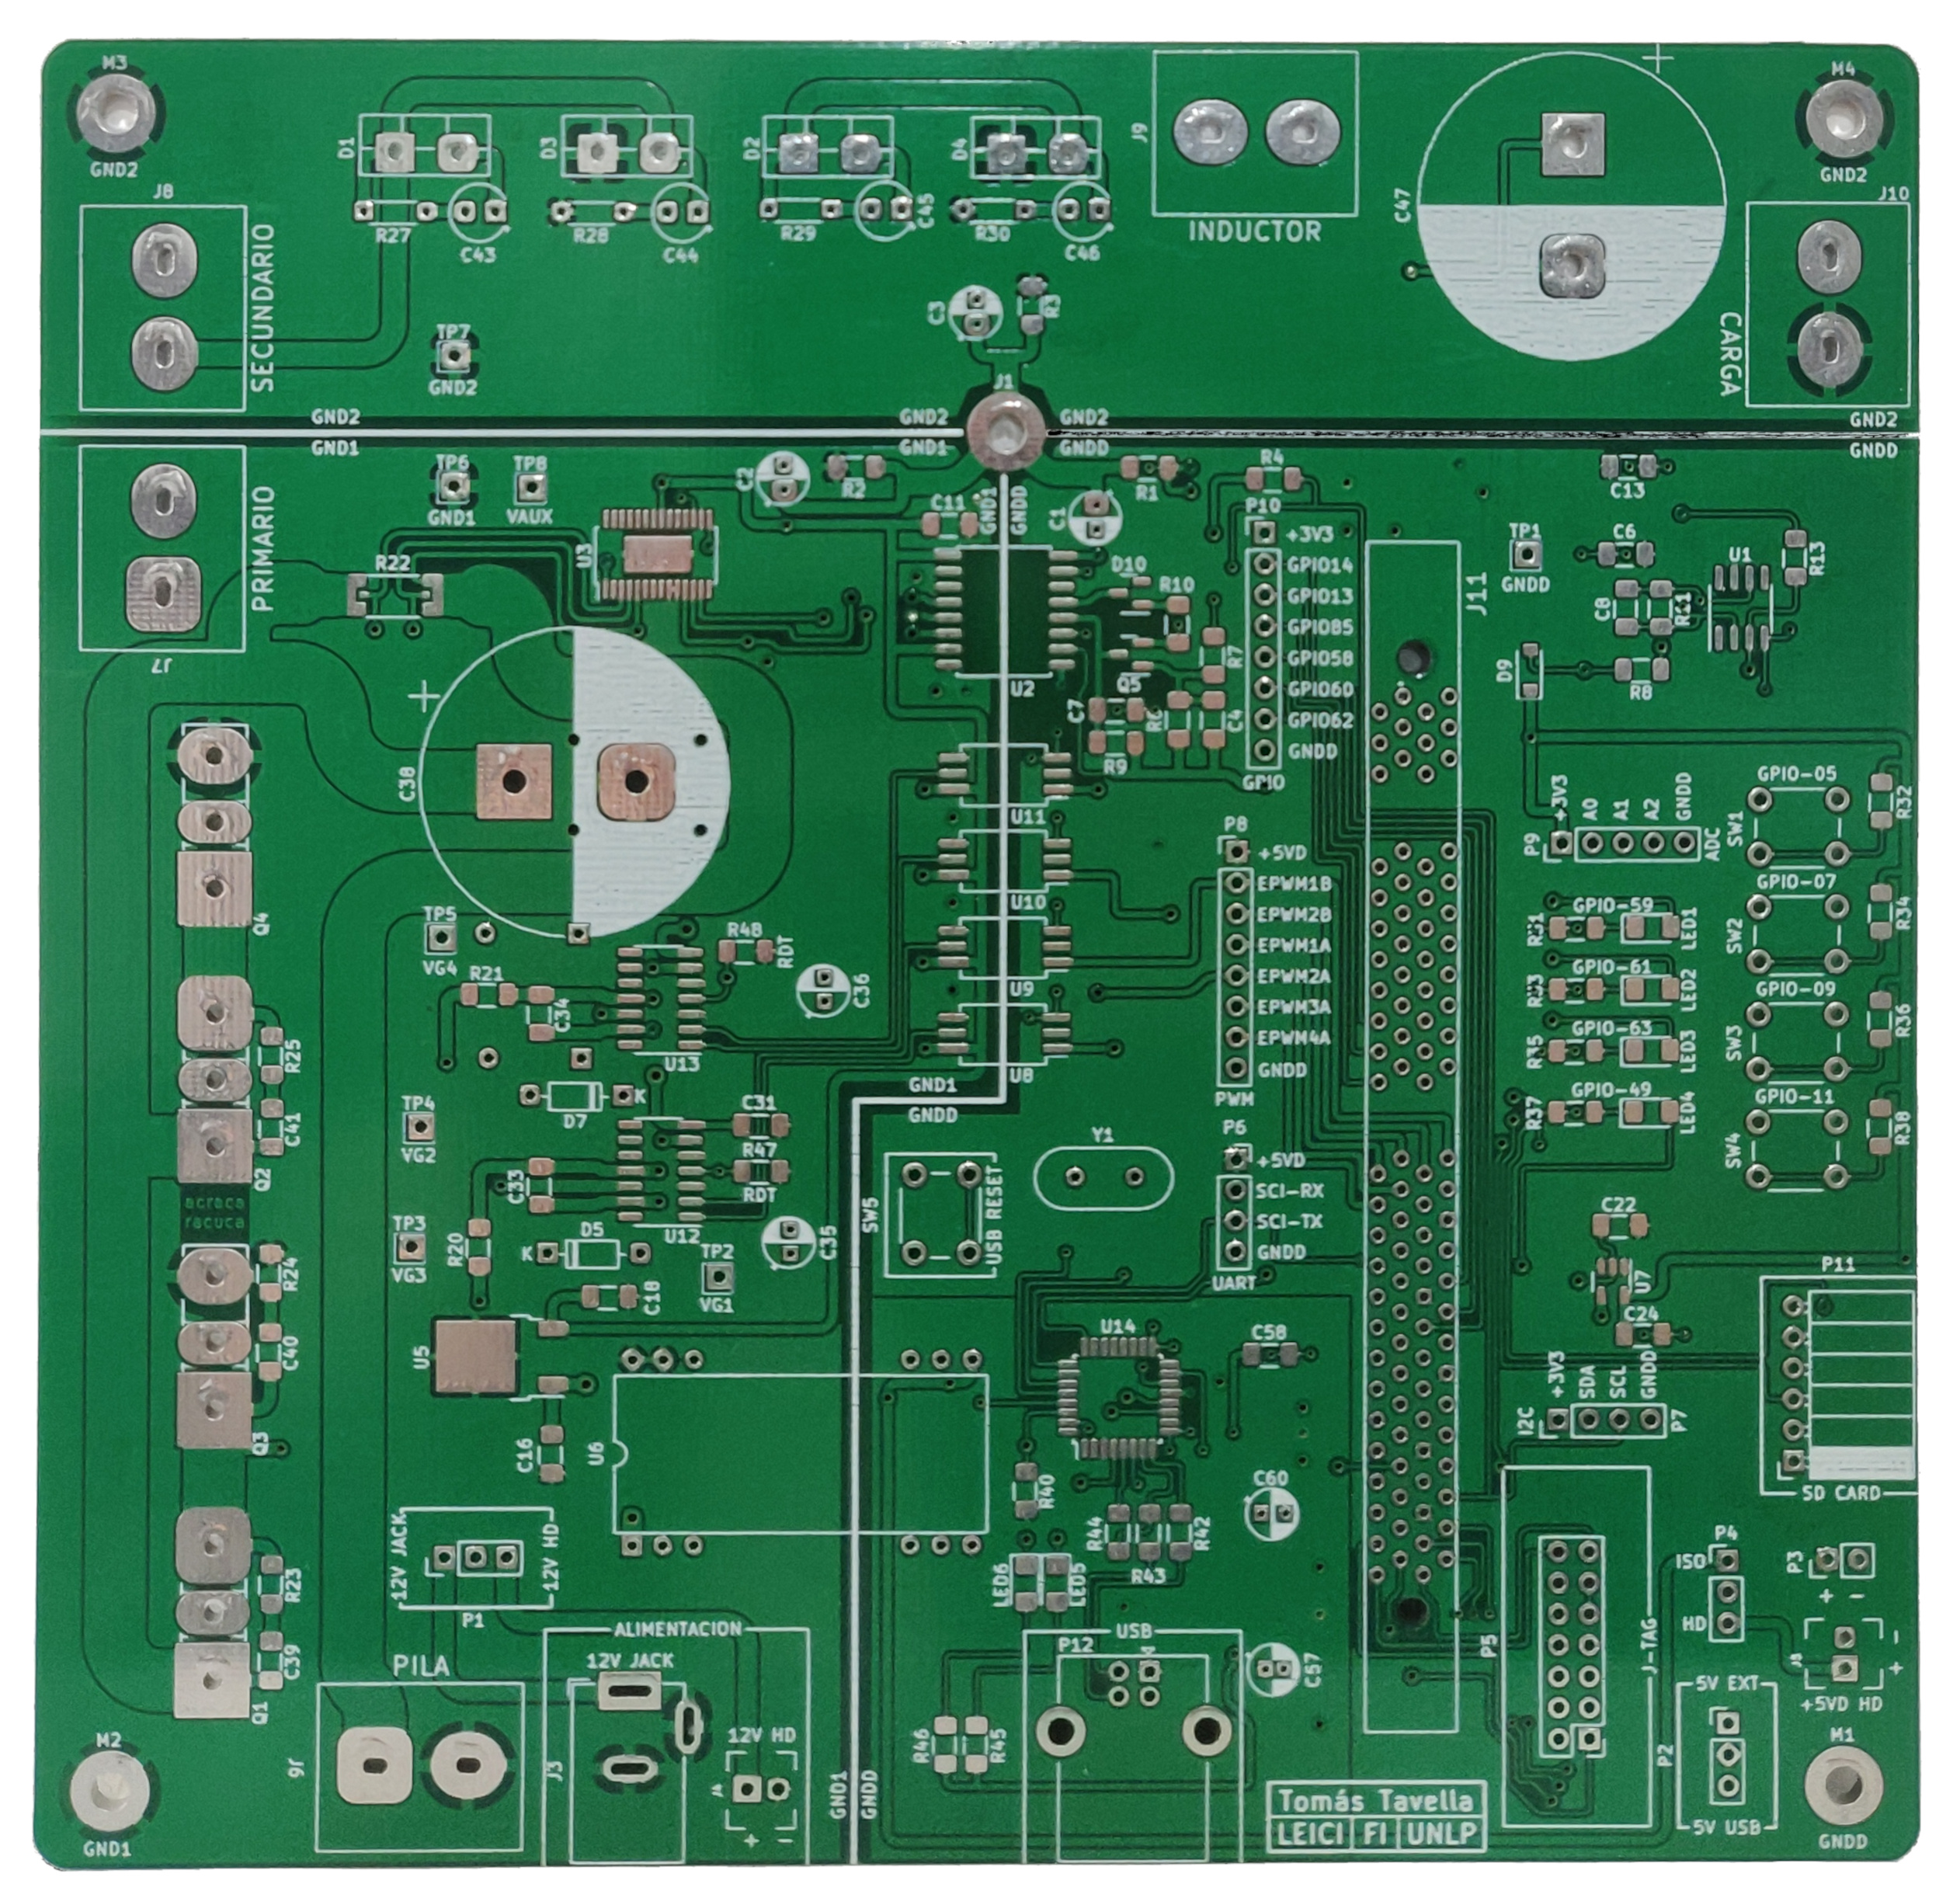
\includegraphics[scale=0.12]{Imagenes/Placa Fisica.jpg}
    \caption{Implementación física de la placa de circuito impreso diseñada, vista desde su capa superior.}
    \label{fig:placa_fisica}
\end{figure}

Adicionalmente, a lo largo de la realización de este trabajo se adquirieron una amplia gama de conocimientos, útiles en el ámbito contemporáneo de diseño e implementación de circuitos. Se aprendió a utilizar una suite de software EDA, herramienta sumamente importante para la implementación de circuitos impresos de cualquier tipo. Además, se adquirieron conceptos y técnicas generales de implementación de circuitos en PCB, como las formas de ruteo de pistas de cobre, el cálculo de los anchos necesarios de estas pistas, la obtención y edición de footprints para ajustarse a los componentes, entre otros.\\